\documentclass{layout/tudelft-report}

\addbibresource{bibliography/references.bib}
\usepackage{tikz-timing}[2009/05/15]
\usepackage{longtable}
% Define Notation commands
% Underlined vectors:
\def\x{\underline{x}}
\def\u{\underline{u}}
\def\p{\underline{p}}
\def\v{\underline{v}}
\def\q{\underline{q}}

% Control surface deflections
\def\del{\delta_{e}}
\def\dail{\delta_{a}}
\def\drud{\delta_{r}}

% Cal symbols
\def\H{{\cal H}}
\def\B{{\cal B}}
\def\D{{\cal D}}
\def\I{{\cal I}}
\def\N{{\cal N}}
\def\O{{\cal O}}
\def\U{{\cal U}}
\def\A{{\cal A}}
\def\S{{\cal S}}
\def\X{{\cal X}}
\def\R{{\cal R}}
\def\Z{{\cal Z}}
\def\P{{\cal P}}
\def\M{{\cal M}}
\def\L{{\cal L}}
\def\T{{\cal T}}

% Mathbb characters
\def\TT{{\mathbb{T}}}

% Parameter vectors
\def\k{{k}}
\def\w{{w}}

% Greek symbol shorthands
\def\eps{{\epsilon}}
\def\th{{\theta}}

\def\simc{\!\sim\!}
\def\ind#1{{\mathbbm 1}_{#1}}
\def\la{($\lambda$)\xspace}
\def\vpi{v_\pi}
\def\vstar{v_*}
\def\qpi{q_\pi}
\def\qstar{q_*}

% || || 
\renewcommand{\norm}[1]{\left\Vert#1\right\Vert}

% || ||_p
\newcommand{\Lpnorm}[1]{\left\Vert#1\right\Vert_{p}}

% | |
\renewcommand{\abs}[1]{\left| #1 \right|}

% :=
\newcommand{\bydef}{\coloneqq}

% Curlies { . }
\newcommand{\curlies}[1]{\left\{ #1 \right\}}

% Set { . }
\newcommand{\set}[1]{\left\{ #1 \right\}}

% Square brackets [ . ]
\newcommand{\sqBrackets}[1]{\left[ #1 \right]}

% Tuple < . >
\newcommand{\tuple}[1]{\left\langle #1 \right\rangle}



% Equal by distributions:
\newcommand{\distrequal}{\overset{\mathcal{D}}{=}}

% Equal by distributions by definition:
\newcommand{\distrbydef}{\overset{\mathcal{D}}{\coloneqq}}

% Probability:
\renewcommand{\Pr}[2][]{
    \mathbb{P}_{#1}\sqBrackets{#2}
}

% Expectation:
\newcommand{\E}[2][]{
    \mathbb{E}_{#1}\sqBrackets{#2}
}

% Gradient:
\def\gradient{\nabla}

% Real numbers:
\def\Real{\mathbb{R}}

% Transpose:
\def\Tr{^\top}

% Nicer conditional:
\def\Vertical{~\vert~}

% argmax
\newcommand{\argmax}[2]{
    \underset{#1}{argmax}\left( #2 \right)
}

% log
\renewcommand{\log}[1]{\textsf{log}~#1}

% Theorems and stuff
\newtheorem{theorem}{Theorem}[section]

% Degrees
\renewcommand{\deg}{\si{\degree}\xspace}

% Short-hand commands
\def\HINF{{$H_{\infty}~$}}

\def\QLAMBDA{{$Q(\lambda$)-learning}}

\renewcommand{\max}[1]{
    \underset{#1}{\text{max}}~
}

\renewcommand{\argmax}[1]{
    \underset{#1}{\text{argmax}}~
}

\newcommand{\epsgreedy}[1]{
    \epsilon\text{-}greedy\left( #1 \right)
}

\newcommand{\clip}[1]{
    \text{clip}\left(#1\right)
}

% \num command to pretty print 1e-5
\def\num#1{\numx#1}\def\numx#1e#2{{#1}\mathrm{e}{#2}}


% Nomenclature
\makenomenclature

\begin{document}

    \frontmatter

    % Thesis Parameters
    \title{Sensors and Communication Systems of the manikin}
    \subtitle{Firmware Validation and Integration.}
    \author{Richard Kroesen en Victor Hogeweij}
    \subject{Project Report}

    % Cover Page
    \makecover
    
    % Title Page
    \begin{titlepage}

\begin{center}

%% Print the title
{\makeatletter
\largetitlestyle\fontsize{45}{45}\selectfont\@title
\makeatother}

\bigskip

%% Print the subtitle
{\makeatletter
\vspace{12mm}
\ifdefvoid{\@subtitle}{}{\largetitlestyle\fontsize{20}{20}\selectfont\@subtitle}
\makeatother}

\bigskip
\bigskip

by

\bigskip
\bigskip

%% Print the name of the author
{\makeatletter
\largetitlestyle\fontsize{25}{25}\selectfont\@author
\makeatother}

\bigskip
\bigskip



\vfill

%% Print some more information at the bottom
\begin{tabular}{ll}
\textit{Opdrachtgever en begeleiders}:      & \\
Skills Begeleider:                          & Kirsten Voncken \\ 
Opdrachtgever:                    & Johan Korten \\
Opleiding:                          & Embedded Systems Engineering \\
Instituut:                          & School of Engineering and Automotive, Hogeschool Arnhem-Nijmegen\\
Project looptijd: & Februari, 2023 - Juli, 2023 \\
Student number: & 2107733 (Victor Hogeweij) en 1663339 (Richard Kroesen)\\
\end{tabular}

\vspace*{1cm}


\vspace*{2cm}
  \begin{center}
    \begin{tabular}{lcr}
      Embedded Systems Engineering & $\cdot$ & HAN University of Applied Sciences
    \end{tabular}
  \end{center}

\end{center}

\end{titlepage}

    
    % Copyright Page
    \begin{flushleft}
  \vspace*{15cm}
  \vspace*{\stretch{3}}
  \thispagestyle{empty}
  \noindent%
  
\includegraphics[width=55mm]{layout/han/HAN_logo.png}\\  
  Copyright \copyright\ Richard Kroesen en Victor Hogeweij, 2023 \\
  All rights reserved.
  \cleardoublepage
\end{flushleft}

    \chapter{Summary}

The project aims to enhance CPR training by implementing an automated real-time feedback system in a modular baby CPR doll. The objective is to integrate and test subsystems, establish firmware version control, and ensure software quality through thorough testing. The architecture design outlines system structure, data flow, and connectivity interfaces. The technical design incorporates protocols for communication and selects the Arduino framework for development. The deliverables include a feature-rich firmware and accompanying documentation. Testing and validation are performed using various methodologies, ensuring system reliability. The project achieves significant milestones, including modular firmware, comprehensive testing, and essential data acquisition software modules. Overall, the project lays a strong foundation for CPR training test instrument system.
    
    % Make a preface page
    \chapter*{Preface}
This project is a big opportunity to develop better skills in software, hardware and documentation. The goal of the project is developing a baby sized CPR doll to help nurses practice their CPR skills.\\ The project has been launched a few years ago, which means that most of the ground work was already done and the (global) working principle of the system is already defined and well documented. \\\\The focus of this report will be on the details of implementing the globally laid out system and on testing the units of this system. Which will be a big challenge and learning opportunity, since neither Richard nor Victor has done something with unit-testing and hardware integration testing, besides running basic examples. 
    
    % TOC, Nomenclature, List of stuff
    \tableofcontents    
    \printnomenclature
    \listoffigures
    \listoftables

    %% Report
    \mainmatter
    % Abbreviations
\nomenclature[A]{CPR}{cardiopulmonary resuscitation}
\nomenclature[B]{SBC}{Single-board Computer}

% Greek letters

% Aerospace stuff


    \chapter{Introduction}
\label{chapter:intro}

\section{Background}
Each year cardiac arrests account for more than thirty percent of mortality worldwide. Since
early cardiopulmonary resuscitation (CPR) is an important factor in survival of a cardiac arrest,
it would be beneficial for a large population to have up-to-date CPR skills. This project tries to
improve quality of CPR training by proposing a system for automated real-time feedback.
Existing systems for CPR training all have their limits in providing desired feedback to a large
group of CPR learners and that is why a novel modular and open patient simulation system was
developed. \cite{jakortenmsc}\\\\
Due to the modular characteristic of this open patient simulation system, the system can be used from baby to grown up CPR training. 
For this project the goal is to implement this modular system in a baby CPR doll (also referred to as a manikin).
\section{Objective for this term project}
The previous student groups which worked on this project have made quite some progress in reading the compression, flow and finger position sensors embedded in the manikin.
\\However the code for reading the sensors are still separate programs which need to be integrated in to one big program. Besides this problem, we have to solve the varying code quality of those programs and also verify the output of these programs in a practical and scientific manner.\\\\
The objectives of this project are:\\
a). To rework every piece of written code to match code styling standards and software engineering good practices.\\
b). To integrate the reworked code in to one big program.\\
c). To test the integrated code with software and hybrid software tests (using simulators, test benches and software unit-tests).\\
d). To learn to test and integrate code 

    % Parts can have epigraphs to add notes
    \epigraphhead[650]{}
    \chapter{Functional Design}
\label{chapter:intro} 
The functional design provides a detailed description of how the system will operate and how it adds value towards the current total system solution.
\newline
This chapter describes what the system's requirements and specifications. Future more system features, and finally also the system interactions are documented.

\section{Functional Requirements}
\begin{tabular}{ |c|l|c|c| } 
 \hline
 Requirement ID & Requirement & MoSCoW \\ 
 \hline
 \hline
 F1    & Every sensor in the system has to provide an validated value  & CH \\ 
       & (within specifications listed in the datasheet of the sensor) to the sensorhub.  &  \\
       &                                                                                  &  \\
\hline
 F1.1  & Validation of the sensors has to be done with a calibrated                       & CH \\
       & reference or testing device.                                                     &   \\
\hline
 F2    & A Test suite has to be designed to validate and collect sensor results.          & CH \\
 \hline
 F2.1  & The Test suite has to have a plotting feature                                    & SH \\
 \hline 
 F2.2  & The Test suite has to support exporting harvested sensor data to an excel or csv file & SH \\
 \hline
 F3    & Data from the sensors has to be stored & MH\\
       & to be used later for determining whether CPR was successful.  & \\
\hline
 F4    & The software design has to support the currently chosen and constructed & MH  \\
       & sensor modules used in the Manikin & \\
 \hline
 F4.1  & The software design has to support the time of flight sensor & MH \\
       & hardware chosen and constructed by previous groups. & \\
\hline
 F4.2  & The software design has to support the pressure sensor & MH \\
       & hardware chosen and constructed by previous groups. & \\
\hline
 F4.3  & The software design has to support the differential pressure sensor & MH \\
       & hardware chosen and constructed by previous groups. & \\
\hline
 F4.4  & The software design has to support the finger position sensor & MH \\
       & hardware chosen and constructed by previous groups. & \\
\hline
 F5    & The data bus between the sensorhub and the mainbord has to use & SH\\
       & a testable and extendable data protocol. &   \\
 \hline
 F5.1  & The data protocol has to be implemented using the i2c bus protocol. & MH \\
 \hline
 F6    & The software design has to implement a post (Power-On System Test) procedure. & WNH \\ 
 \hline
\end{tabular}

\section{Non-Functional Requirements}
\begin{tabular}{ |c|l|c|c| } 
 \hline
 Requirement ID & Requirement & MoSCoW \\ 
 \hline
 \hline
 NF1    & The software design has to implement software engineering best practices.  & MH \\
 \hline
 NF2    & The software design has to use an consistent code style & MH \\
 \hline 
 NF3    & The software-, hardware-design and documentation are stored  & MH \\
        & in public GitHub repository's & \\
\hline
 NF4   & Software unit tests have to be constructed to test the software & MH\\
 \hline
\end{tabular}
\section{Design Constraints}
There are a few design constraints related to this project.\\ 
These constraints are either related to technical constraints or time related constraints. \\ This project is financed and backed by the school and most of the hardware is mostly handled by Johan and the IPS students, therefore there are no financial or organizational constraints.
\subsection{Technical design constraints}
There are multiple constraints in this category, due to the hardware and software decisions made by Johan and the previous project term groups. These constraints where easily pointed out and have helped with creating the functional requirements. To help analyse how much extra time a design constraint will take to tackle, a ranking system was added to the table.\\
\begin{tabular}{|l|c|}
\hline
    Constraint & Rank \\
               & (1 meaning low time effort, 10 meaning big effort) \\
    \hline\hline
     Previous groups have chosen the Arduino framework. & 5\\
     But no research was done on the subject of \\frameworks for the samd series. Which probably means that \\ custom software implementations for hardware functions \\have to be made. Due to Arduino's limited support.\\ & \\
     \hline
     Due to the varying skillset of the upcoming project term groups. & 3\\
     The code written has to be easy to understand. \\ Which might limit us in the use of tools or software frameworks.\\
     \hline
     
     
     
     
\end{tabular}

\subsection{Time related constraints}
    \chapter{Architecture design}
\label{chapter:intro}
This chapter gives an overview of the system design on the highest-level. Abstraction is used to cover the details which are not essential to outline what the system does and how it works in the big lines. \newline
The architecture outlines the structure, components, and interactions of a software or hardware system. It is an essential element to understand the system. 

\section {Architecture Diagram}

\section {Data Flow}
\section {System Dependencies}

\section {System interfaces}

\chapter{Technical Design}
This chapter translates the functional and the architecture into the real-world engineering implementation. 
\section{Class Diagram}
\section{Hierarchical/Abstraction Overview}
\section{Protocols Highlights}
For the details of the protocols, please consult the appendix. This section only covers the basics for understanding. and awareness of existence.  
\section{Engineering Decisions}
-- Here we should document things like why we are using I2S, SPI and testing framework Google Testing. 

    \chapter{Technical Design}
This chapter translates the functional and the architecture into the real-world engineering implementation. 

\section{Protocols Highlights}
For the details of the protocols, please consult the appendix. This section only covers the basics for understanding. and awareness of existence.  \\
\subsection{SPI Slave protocol}
This protocol is used for the communication on the internal communicationbus of the mainboard (between the Raspberry Pi and the SAMD51).\\
\subsubsection{SPI interface}
This is the only communication bus in the manikin which utilizes a SPI data interface. SPI is a synchronous communication interface. The standard for the SPI interface specifies the rules and requirements for data transfer between devices. It provides a framework for synchronous, full-duplex communication between a master device and one or more slave devices.\\\\
With a SPI bus, communication is established between a master device (often a microcontroller) and one or more slave devices. The master device controls the communication by sending and receiving data to and from the slave devices.\\\\
The SPI bus uses a set of wires or lines for communication:\\\\
- SCLK (Serial Clock): This line carries a clock signal generated by the master device. It synchronizes the data transfer between the master and the slave devices.\\
- MOSI (Master Output, Slave Input): This line is used by the master device to send data to the slave device(s).\\
- MISO (Master Input, Slave Output): This line is used by the slave device(s) to send data back to the master device.\\
- SS/CS (Slave Select/Chip Select): This line is used to select a specific slave device for communication when multiple slaves are connected to the SPI bus. The master device activates this line for the desired slave device before sending or receiving data.\\\\
The data transfer on the SPI bus occurs in a full-duplex manner, meaning that data can be sent and received simultaneously. The master device initiates the data transfer by sending clock pulses on the SCLK line.\\ For each clock pulse, a bit of data is transferred on the MOSI line from the master to the slave, while the MISO line carries the data from the slave to the master.\\\\

\subsubsection{Slave protocol}
The SPI standard only defines the data transfer between devices but not the protocol on top. This has to be created by the manufacturer of the slave device. Therefore for this project, a slave protocol had to be built which can be implemented on the SPI interface.\\\\
The details of this protocol can be read in appendix \ref{appendix::SPI_SLAVE_PROTOCOL}. The chosen design was made with data integrity in mind. That means that both written and read bytes on the databus are validated with a maxim-CRC8 algorithm. If the integrity check fails, data can be requested using the sequence number. \\\\
The slave protocol designed looks a lot like the I2C slave protocol used between the sensor/power/actuator- hubs and the mainboard. This was by design and makes the implementation of the protocols a bit easier as the software could now be written in a more generic manner. \\
\pagebreak
\subsubsection{Features}
This protocol can be used to set and get: the sensor types, sampling rates of the sensors, status and the sensor data of the system. \\ This is done by writing and reading to the registers of the slave device (in this case sensor-, actuator- and powerhub). The registers are defined in appendix \ref{appendix::SPI_SLAVE_PROTOCOL}.

\subsection{USB Service protocol}
This protocol is used for the communication from the hubs to an external computer over (VCOM) USB.\\ This can be used in conjunction with other mentioned dataprotocols and adds another communication functionality to the hubs.\\

\subsubsection{VCOM interface}
This protocol uses the VCOM data interface, which is a virtual COM port over USB. The VCOM port can then be used like a real UART connection. Providing a lot of flexibility since we have dont have to worry about the hardware side of UART. To read more about the UART connection settings for the VCOM port read appendix \ref{appendix::usb_service_protocol}.

\subsubsection{Service protocol}
To make things easier and to emulate a serial console the messages send over UART for the protocol is in plain ascii and represent abbreviated English words as commands. The usage of the service protocol is similar to the usage of a linux/unix commandline. Status and sensor readings are send in json format over the console. The left over commands return confirmations in plain text with \texttt{!ERR} for errors and \texttt{!OK}. For the full usage and explaination, take a look at appendix \ref{appendix::usb_service_protocol}.

\subsubsection{Features}
The features of this protocol are very similar to the SPI slave protocol. This protocol can be used as a replacement or in conjunction with the SPI slave protocol and will provide the same information and options. The only big difference between this and the SPI protocol is that this protocol is human comprehensible and doesn't need scripts or an application to harvest system parameters. 


\section{Engineering Decisions}
The Engineering Decisions section is meant to document crucial choices which have consequences or limitations for the future of the project life cycle. \\ 
This section serves as a comprehensive record of the key decisions made by the development team, providing valuable insights into the reasoning, considerations, and trade-offs that influenced the chosen path.\\\\
Lastly this is also the section for reference to make iterations, enhancements and/or maintenance easier.
\subsection{Software Framework}
The framework used on the hubs and the mainboard use the Arduino framework. The software delivered by the previous groups was based on the Arduino framework and was non-functional. Which meant it needed a rewrite. We have considered using another framework like zephyr or Microchip ASF. \\To test these frameworks we have constructed the following requirements:\\
FrameworkSpec-1[MH] The framework has to be easy to learn/use for the beginning programmer. \\
FrameworkSpec-2[SH] The framework can be easily reconfigured to support different platforms (SAMD21/SAMD51).\\
FrameworkSpec-3[MH] The framework can be configured reliably.\\
FrameworkSpec-4[SH] The framework supports all hardware peripherals of the SAMD21/51\\
\pagebreak
\subsubsection{Microchip ASF}
Microchip ASF, also known as the Microchip Advanced Software Framework, is a collection of libraries and drivers provided by Microchip Technology. It is designed to simplify and accelerate the development of applications for Microchip microcontrollers and microprocessors. \\\\
\textbf{Advantages of Microchip ASF:} \\\\
+ \textbf{Comprehensive library support:} Microchip ASF offers a wide range of libraries that provide ready-to-use software components and drivers for various peripherals and functionalities. These libraries cover areas such as communication interfaces (e.g., UART, SPI, I2C), timers, interrupts, file systems, and more. By using these libraries, developers can save time and effort by not having to implement low-level functionality from scratch.\\ 
+ \textbf{Device abstraction and portability:} Microchip ASF provides an abstraction layer that hides the hardware details of different Microchip microcontrollers and microprocessors. This allows developers to write code that is portable across multiple devices, reducing the effort required to adapt applications to different hardware platforms. \\
+ \textbf{Integration with development tools:} Microchip ASF integrates with Microchip's development tools, including the MPLAB X IDE and MPLAB Harmony framework. \\
+ \textbf{Extensive documentation and support:} Microchip ASF is backed by comprehensive documentation and resources, including user guides, application notes, and example projects. This helps developers understand and utilize the framework effectively. Additionally, Microchip offers technical support and an active community where developers can seek assistance and share knowledge. \\\\
\textbf{Disadvantages of Microchip ASF:}\\\\
- \textbf{Learning curve and complexity:} Microchip ASF can be complex, especially for beginners or developers new to Microchip microcontrollers. The extensive range of libraries and the underlying abstraction layer may require a learning curve to understand and utilize effectively. However, the availability of documentation and support can help mitigate this challenge. \\
- \textbf{Hardware dependency:} Microchip ASF is tightly coupled with Microchip microcontrollers and microprocessors. It may not be directly compatible with other hardware platforms or microcontrollers from different manufacturers. This can limit the flexibility and portability of applications developed using ASF. \\
- \textbf{Limited customization options:} While Microchip ASF provides a wide range of pre-built libraries, customization options may be limited compared to building the software from scratch. Developers may face constraints in tailoring the software to their specific requirements or adding new features that are not supported out-of-the-box.


\pagebreak
\subsubsection{Zephyr RTOS}
Zephyr RTOS is an open-source operating system designed specifically for resource-constrained embedded systems. It provides a software framework that enables developers to build real-time applications for a wide range of devices. \\\\
\textbf{Advantages of Zephyr RTOS: }\\\\
+ \textbf{Real-time capabilities}: Zephyr RTOS is designed to handle real-time requirements, where precise timing and responsiveness are critical. It provides mechanisms for tasks and interrupts to be scheduled and executed with predictable timing, making it suitable for applications that require precise control and quick response times. \\
+ \textbf{Scalability}: Zephyr RTOS is highly scalable and can be used on a wide range of devices, from low-power microcontrollers to more powerful boards. It offers a modular architecture that allows developers to choose and configure only the components they need, optimizing resource usage and making it adaptable to different hardware platforms. \\
+ \textbf{Open-source and active community}: Zephyr RTOS is an open-source project, which means the source code is freely available for anyone to use, modify, and contribute to. It benefits from an active community of developers who collaborate, share knowledge, and provide support. This fosters continuous improvement, bug fixes, and the addition of new features. \\
Support for multiple architectures: Zephyr RTOS supports a wide range of processor architectures, including ARM, RISC-V, x86, and more. This allows developers to use the operating system on various hardware platforms, giving them flexibility and choice when selecting the right hardware for their projects. \\\\
\textbf{Disadvantages of Zephyr RTOS:} \\\\
- \textbf{Learning curve}: Zephyr RTOS may have a steeper learning curve compared to simpler frameworks like Arduino. It requires familiarity with concepts related to real-time systems, such as task scheduling, interrupts, and synchronization mechanisms. However, the availability of documentation and community support can help overcome this challenge. \\
- \textbf{Device-specific configurations}: Since Zephyr RTOS supports multiple hardware platforms, configuring and setting up the operating system for a specific device may require some effort. Device-specific configurations may involve understanding the hardware details and configuring drivers and peripherals accordingly. \\
- \textbf{Hardware limitations}: While Zephyr RTOS is highly scalable, it may not be suitable for extremely resource-constrained devices with very limited memory or processing power. The additional functionality and flexibility provided by an operating system come with some overhead in terms of memory and performance requirements.
\pagebreak
\subsubsection{Arduino}
The Arduino framework refers to the software and libraries that enable programming and interacting with Arduino boards.\\\\
\textbf{Advantages of the Arduino framework: }\\\\
+ \textbf{Simplified programming:} The Arduino framework uses a simplified programming language based on C/C++. It abstracts many low-level details and provides easy-to-use functions and libraries, making it accessible to beginners with little or no programming experience. \\
+ \textbf{Rich library ecosystem:} The Arduino framework comes with a vast library ecosystem. These libraries contain pre-written code that can be easily incorporated into the project, saving time and effort. Libraries exist for various functionalities like controlling motors, reading sensors, and communicating with other devices.\\
+ \textbf{Community support:} Arduino has a large and active community of users. This means there are numerous online resources, forums, and tutorials available where you can seek help. The community support makes it easier to overcome challenges. \\
+ \textbf{Cross-platform compatibility:} The Arduino framework is compatible with multiple operating systems, including Windows, macOS, and Linux. This allows you to work on your projects using the computer you're most comfortable with, without being restricted to a specific platform. \\\\
\textbf{Disadvantages of the Arduino framework:} \\\\
- \textbf{Limited low-level control:} The Arduino framework abstracts many low-level details to make programming easier. While this is advantageous for beginners, it can be limiting for advanced use cases which need to be tightly integrated with the underlying hardware. \\
- \textbf{Memory limitations:} Arduino boards have limited memory resources. The Arduino framework's simplicity and ease of use come at the cost of increased memory usage. This can be a constraint for projects that require complex algorithms or extensive data storage. \\
- \textbf{Hardware dependencies:} The Arduino framework is tightly integrated with Arduino boards. While this ensures compatibility and ease of use, it may not be suitable for projects that require different hardware platforms or specialized components. \\
\pagebreak
\subsubsection{Conclusion}
To help with choosing the right framework for this project we used a table with each column representing a requirement.\\
We still stuck to arduino due to the low skill needed to understand and write programs based on the arduino framework. The disadvantage of limited low-level control can be mitigated by creating low-level libraries for certain hardware peripherals. The memory limitations and hardware dependencies can be solved by having enough RAM/FLASH space and by minimizing software dependencies on arduino in the software design.

\begin{center}
\footnotesize
\begin{longtable}{|m{10em}|m{10em}|m{10em}|m{10em}|m{10em}|}
    \hline
    Framework & easy to use/learn & easily reconfigurable & reliable & supports all hardware \\ \hline
    Zephyr & Steep learning curve, uses non-standard way of initializing and utilizing hardware peripherals & Yes and no, When the platform is supported and all drivers used are available to the platform then yes it is easy to reconfigure. If not the case the answer is no & Yes, when used correctly it functions very reliably, gives compiler warnings when used incorrectly & No, most of the hardware functions are supported. Additional hardware drivers have to be written manually \\ \hline
    ASF & Moderate learning curve, needs knowledge of the hardware to use. & No, due to the easy to use API it is very tightly coupled, doing a lot of things under the hood which differ for each platform & No, when making mistakes this framework doesn't give any warnings and it lets the user easily misconfigure peripherals & Yes, it is written by the manufacturer of the mcu series used in this project, and supports all the hardware functions of the SAMD21/51\\ \hline
    Arduino & Beginner friendly & It is written to be cross platform and uses wrappers under the hood to provide the same functionality for each platform. & Yes, when using first-party libraries the arduino framework can be reliable. & No, it doesn't support all peripherals of the SAMD, because Arduino is written to be as generic as possible and only support features which are on the Arduino boards \\ \hline
\end{longtable}
\end{center}
\subsection{Style guide}
Requirement NF2 in chapter \ref{chapter:requirements} states that a consistent code style needs to be applied to current and new code. After a thorough look through the currently available code styles and decided to use the Google Style guide. We chose this one since it isn't too limiting for usage on embedded systems. It does still allow the usage of old c-style functions instead of the standard lib which is very resource intensive for embedded systems. And it would mix well with our testing framework which also utilizes the Google Style guide.
\subsection{Version control system}
Requirement NF3 in chapter \ref{chapter::requirements} states that the code, hardware and documentation needs to be stored in public GitHub repository's. Our project client made a GitHub Organization and gave permission to create repository's. \\\\
We created the following repository's:\\
- Manikin Software -> To store (firmware) code in for each manikin component and complementary tools (like data harvesting scripts) (SensorHub, ActuatorHub, PowerHub, scripts) \\
- Manikin Hardware -> To store all the hardware designs made by our client and previous project groups. \\
- Manikin Software Libraries -> To store loosely coupled libraries which act as wrappers or implement low level features not offered by the arduino framework. \\\\
The repository's which contain code also contain several automatically ran GitHub workflows which check the code consistency and whether the code compiles. This helps when reviewing each others code in pull requests as it gives an indication of the code quality.




    \epigraphhead[650]{}
    \chapter{Deliverables Description}
This chapter gives an overview of the Manikin firmware. The objective is to inform and explain how and what the current version (release 1.0.0) of the firmware does.
\section{Firmware Functionality Highlights}
The current release version 1.0.0 is able to do this:
\begin{itemize}
  \item Exception handling using the Serial console.
  \item Saving and reading the unique device identifier from the onboard external flash memory (can be done using usb serial console, SETID and STATUS command)
  \item Set the sensortype for each sensorport from the usb serial console using the SETPORT command.
  \item Reading sensor value's using the STREAM command from the usb serial console.
  \item Set the sample rate in milliseconds from the usb serial console (using SETSR command).
  \item Get the module status and identifier using the STATUS command in the usb serial console.
  \item Build to easily expand the current commandset and adding more methods to the usb serial service console.
  \item HELP command for showing manual usage in serial console.
  \item Is able to use the compression, ventilation and finger position sensor using the sensor libraries from Manikin Software Libraries.
  \item Has functionality for running unit tests.
  \item Has custom board configuration files for the sensorhub module.
  \item Modular software solution to enable easy integration of other sensors.
\end{itemize}

\section{Software Libraries}

\subsection{GPIO}
The GPIO library is a minimal library written to drive the GPIO peripheral of the SAMD51 and SAMD21. The functions do not depend on third-party libraries and uses the internal peripheral registers of the SAMDxx microcontroller.\\\\
The following functionality is supported by this library: \\
- Setting pin states \\
- Toggling pin states \\
- Setting pin input/output states \\
- Linking pin functions to pins using the internal pinmux \\
- Setting pin sink/drive current \\
- Setting pin input sampling mode (continuous/on-demand) \\

\subsection{I2C Master}
The I2C Master is an I2C wrapper which wraps Arduino Wire library to a simplified universal interface. This way all the dependent sensor libraries can easily be ported to another platform, by simply replacing the I2C wrapper with a new wrapper using the platform/oem specific functions.
\subsection{USB service protocol}
The USB service protocol is a library written to emulate a command-line like interface over the VCOM port of the SAMD21/SAMD51. The library uses the Arduino Serial library and FreeRTOS as its foundation. The Arduino Serial library is used to communicate over the VCOM port and FreeRTOS provides easy task-switching. \\
When using the library, a background task is created to  listen for new incoming characters on the VCOM port. When an enter is detected a linear search is performed using strcmp to check if the command is found within the service protocol command and callback struct array.
\subsection{SPI Slave}

\subsection{Sensors}

\subsection{Logger}
\subsubsection{Flash Logger}

\subsubsection{Serial Logger}

\subsection{Exception}






\section{Additional Documentation}
The technical and most up-to-date documentation could be found on the GitHub organization page. 

\section{Data File Script Save}
For the purpose of logging data from the stream, a Python script is employed. This versatile script effectively converts the JSON terminal stream into a format that is more suitable for analysis and further processing.

    \chapter{Verification and Validation}
\label{chapter:vv}


    \epigraphhead[650]{}
    \part{Conclusion}
    \label{part:closure}

    \chapter{State-of-Art}
\label{chapter:conc}
Where did the development of the embedded systems landed? What is realised, and finished etc. 
The main question that this chapter answers is: where did the embedded systems engineering development land? What is the state of the delivered work. What is realised and could be assumed to be finished.
\section{Project Results}
This section lists the modules or parts that are realised. \\
In general this is the contribution that this project had:\\
\begin{itemize}
    \item Modular firmware with proper development organizational version control.
    \item Version controlled development environment with code standards.
    \item Crucial data acquisition software modules tested.
\end{itemize}
Note: The "(RESULT)" indicates whether the result was not a must have in the requirement list.
\begin{table}[hb!]
\begin{tabular}{ |c|l|c|c| } 
 \hline
 Requirement ID & Requirement & Achieved \\ 
 \hline
 \hline
 F1    & Every sensor in the system has to provide an validated value  & (YES) \\ 
       & (within specifications listed in the datasheet of the sensor) to the sensorhub.  &  \\
       &                                                                                  &  \\
\hline
 F1.1  & Validation of the sensors has to be done with a calibrated                       & (NO) \\
       & reference or testing device.                                                     &   \\
\hline
 F2    & A Test suite has to be designed to validate and collect sensor results.          & (YES) \\
 \hline
 F2.1  & The Test suite has to have a plotting feature                                    & (NO) \\
 \hline 
 F2.2  & The Test suite has to support exporting harvested sensor data to an excel or csv file & YES \\
 \hline
 F3    & Data from the sensors has to be stored & YES\\
       & to be used later for determining whether CPR was successful.  & \\
\hline
 F4    & The software design has to support the currently chosen and constructed & YES  \\
       & sensor modules used in the Manikin & \\
 \hline
 F4.1  & The software design has to support the time of flight sensor & YES \\
       & hardware chosen and constructed by previous groups. & \\
\hline
 F4.2  & The software design has to support the pressure sensor & YES \\
       & hardware chosen and constructed by previous groups. & \\
\hline
 F4.3  & The software design has to support the differential pressure sensor & YES \\
       & hardware chosen and constructed by previous groups. & \\
\hline
 F4.4  & The software design has to support the finger position sensor & YES \\
       & hardware chosen and constructed by previous groups. & \\
\hline
 F5    & The data bus between the sensorhub and the mainbord has to use & (NO)\\
       & a testable and extendable data protocol. &   \\
 \hline
 F5.1  & The data protocol has to be implemented using the i2c bus protocol. & (NO) \\
 \hline
 F6    & The software design has to implement a post (Power-On System Test) procedure. & (NO) \\ 
 \hline
\end{tabular}
 \caption{Project requirements results}
 \label{tab:functional_requirements}
\end{table}
This project has achieved the must-haves and some extra goals of the requirements. 
% \section{System Specification}
% Technical parameters specifications of the hub. \\
% Draft of relevant parameters: sampling time (max), buffer size/max samples, memory(ram) usages current, performance?, other limitation factors/absolutes, electrical overview (why not), interfaces overview with corresponding purpose, USB service baud, pcb dimensions, etc

    \chapter{Recommendations}
\label{chapter:rec}

This chapter presents a comprehensive set of recommendations that outline the key areas for future development and advancement of this research project.\\
\subsubsection*{Rec 1: Optimization and Digital Signal Processing}
One significant opportunity for further investigation into the development is digital signal processing application techniques. The current system has a basic although practical digital signal processing. Research into this element of the project could be interesting for offering valuable insights and potential advancements into the feedback of the training.
\subsubsection*{Rec 2: Advancement into Security Standards}
While the current state-of-art may not require immediate security considerations, it is hightly advisable to begin contemplating and implementing security mechanisms. The development team did not implement any security techniques because this was out of project scope.  
\subsubsection*{Rec 3: Hardware Peripherals Optimization and Enhancement}
To optimize the software's performance, a recommended approach is to leverage hardware peripherals such as Direct Memory Access (DMA). By exploring the capabilities of these peripherals and effectively integrating them into the software design, it is possible to achieve significant performance improvements. This optimization strategy enables efficient data transfers, reduces processing overhead, and maximizes the utilization of available hardware resources.
\subsubsection*{Rec 4: Re-design and Development of the mainboard-hub Protocol}
The implementation of the mainboard and the hub communication protocol is not realised during this project. In appendix under section Intranet there is concept for this protocol. However it is not fully worked out. It is highly recommended to use it as a example or starting point, but not to implement directly.

    % Bibliography with numeric style
    \printbibliography[title=References]
    \addcontentsline{toc}{chapter}{References}
    
    % __ Appendix ___
    \appendix
    \part{Appendix}
    \chapter{Entry Induction Guide}

The goal of the Entry Induction Guide is to support next project groups to get started effectively. This guide gives the key takeaways about project specific knowledge(of concepts), skills and tools. 
\\ \\ 
Concept / Draft of things: \\
- CMakeLists (Adviceable)
- GitHub
- read/save for reference the project style guide
- Google Testing framework basics (Required, but not immediately)
- Read/Scan quickly the protocol outlines
- Etc

\section{Guide Assumptions}
The goal of the guide is to be semi-dummy proof, meaning the coverage tries to be wide covered. However due to the audience expectations the guide assumes you are familiar with the following:
\begin{itemize}
    \item Working with GitHub version control: clone, commit, push and pull. Work in branches.
    \item Have experience with VS code IDE. 
    \item Have experience and knowledge about C++.
\end{itemize}

\section{Getting Started}
The previous developers recommend that you start with following this list:
\begin{itemize}
  \item Scan quickly through Architecture Design (chapter 3), look at diagrams to get a general overview and idea of the system. 
  \item Read Firmware Description to understand how and what the firmware does.
  \item Go to the RobotPatient organization GitHub page, and get the release firmware version of Manikin Software, and see if you are able to build and upload to the target device.  
  \item Next step is to decide whether you understand the CMakeLists and Google Testing unit tests. If you have the feeling you lack some knowledge here, go to the corresponding section to find learning/guides/documentation resources.
\end{itemize}
    \chapter{IntraNet}

\section{Registers}
This is the documentation for the IntraNet protocol. The IntraNet protocol is designed for the reliable communication between the hubs and the mainboard. \\\\
All registers are 8 bits (Byte) to keep the protocol relative simple (KISS principle).

\subsection{Status Registers}
Register Tag: 0x00\\
Register size: 8-bits\\
Access: R\\

\begin{tabular}{rp{1.25cm}p{1.25cm}p{1.25cm}p{1.25cm}p{1.25cm}p{1.25cm}p{1.25cm}p{1.25cm}}
Bit &
  7 &
  6 &
  5 &
  4 &
  3 &
  2 &
  1 &
  0 \\ \cline{2-9} 

\multicolumn{1}{r|}{x} &
  \multicolumn{1}{c|}{x} &
  \multicolumn{1}{c|}{x} & 
  \multicolumn{1}{c|}{x} &
  \multicolumn{1}{c|}{x} & 
  \multicolumn{1}{c|}{x} & 
  \multicolumn{1}{c|}{x} &
  \multicolumn{1}{c|}{x} &
  \multicolumn{1}{c|}{x} \\\cline{2-9} 
  
Access &
  R &
  R &
  R &
  R &
  R &
  R &
  R &
  R
\end{tabular}

\subsection{Control Registers}
Register Tag: 0x00\\
Register size: 8-bits\\
Access: R\\

\begin{tabular}{rp{1.25cm}p{1.25cm}p{1.25cm}p{1.25cm}p{1.25cm}p{1.25cm}p{1.25cm}p{1.25cm}}
Bit &
  7 &
  6 &
  5 &
  4 &
  3 &
  2 &
  1 &
  0 \\ \cline{2-9} 

\multicolumn{1}{r|}{x} &
  \multicolumn{1}{c|}{x} &
  \multicolumn{1}{c|}{x} & 
  \multicolumn{1}{c|}{x} &
  \multicolumn{1}{c|}{x} & 
  \multicolumn{1}{c|}{x} & 
  \multicolumn{1}{c|}{x} &
  \multicolumn{1}{c|}{x} &
  \multicolumn{1}{c|}{x} \\\cline{2-9} 
  
Access &
  R &
  R &
  R &
  R &
  R &
  R &
  R &
  R
\end{tabular}


\subsection{Configuration Registers}
Register Tag: 0x00\\
Register size: 8-bits\\
Access: R\\

\begin{tabular}{rp{1.25cm}p{1.25cm}p{1.25cm}p{1.25cm}p{1.25cm}p{1.25cm}p{1.25cm}p{1.25cm}}
Bit &
  7 &
  6 &
  5 &
  4 &
  3 &
  2 &
  1 &
  0 \\ \cline{2-9} 

\multicolumn{1}{r|}{x} &
  \multicolumn{1}{c|}{x} &
  \multicolumn{1}{c|}{x} & 
  \multicolumn{1}{c|}{x} &
  \multicolumn{1}{c|}{x} & 
  \multicolumn{1}{c|}{x} & 
  \multicolumn{1}{c|}{x} &
  \multicolumn{1}{c|}{x} &
  \multicolumn{1}{c|}{x} \\\cline{2-9} 
  
Access &
  R &
  R &
  R &
  R &
  R &
  R &
  R &
  R
\end{tabular}

\subsection{Data Registers}
Register Tag: 0x00\\
Register size: 8-bits\\
Access: R\\

\begin{tabular}{rp{1.25cm}p{1.25cm}p{1.25cm}p{1.25cm}p{1.25cm}p{1.25cm}p{1.25cm}p{1.25cm}}
Bit &
  7 &
  6 &
  5 &
  4 &
  3 &
  2 &
  1 &
  0 \\ \cline{2-9} 

\multicolumn{1}{r|}{x} &
  \multicolumn{1}{c|}{x} &
  \multicolumn{1}{c|}{x} & 
  \multicolumn{1}{c|}{x} &
  \multicolumn{1}{c|}{x} & 
  \multicolumn{1}{c|}{x} & 
  \multicolumn{1}{c|}{x} &
  \multicolumn{1}{c|}{x} &
  \multicolumn{1}{c|}{x} \\\cline{2-9} 
  
Access &
  R &
  R &
  R &
  R &
  R &
  R &
  R &
  R
\end{tabular}

\subsection{Command Registers}
Register Tag: 0x00\\
Register size: 8-bits\\
Access: R\\

\begin{tabular}{rp{1.25cm}p{1.25cm}p{1.25cm}p{1.25cm}p{1.25cm}p{1.25cm}p{1.25cm}p{1.25cm}}
Bit &
  7 &
  6 &
  5 &
  4 &
  3 &
  2 &
  1 &
  0 \\ \cline{2-9} 

\multicolumn{1}{r|}{x} &
  \multicolumn{1}{c|}{x} &
  \multicolumn{1}{c|}{x} & 
  \multicolumn{1}{c|}{x} &
  \multicolumn{1}{c|}{x} & 
  \multicolumn{1}{c|}{x} & 
  \multicolumn{1}{c|}{x} &
  \multicolumn{1}{c|}{x} &
  \multicolumn{1}{c|}{x} \\\cline{2-9} 
  
Access &
  R &
  R &
  R &
  R &
  R &
  R &
  R &
  R
\end{tabular}

\subsection{Error Registers}
Register Tag: 0x00\\
Register size: 8-bits\\
Access: R\\

\begin{tabular}{rp{1.25cm}p{1.25cm}p{1.25cm}p{1.25cm}p{1.25cm}p{1.25cm}p{1.25cm}p{1.25cm}}
Bit &
  7 &
  6 &
  5 &
  4 &
  3 &
  2 &
  1 &
  0 \\ \cline{2-9} 

\multicolumn{1}{r|}{x} &
  \multicolumn{1}{c|}{x} &
  \multicolumn{1}{c|}{x} & 
  \multicolumn{1}{c|}{x} &
  \multicolumn{1}{c|}{x} & 
  \multicolumn{1}{c|}{x} & 
  \multicolumn{1}{c|}{x} &
  \multicolumn{1}{c|}{x} &
  \multicolumn{1}{c|}{x} \\\cline{2-9} 
  
Access &
  R &
  R &
  R &
  R &
  R &
  R &
  R &
  R
\end{tabular}
    \chapter{SPI Mainboard}
\section{Introduction}
For the internal communication bus on the mainboard is a well described datacommunication protocol needed. This document will provide the information needed to implement the datacommunication protocol used on the mainboard in software/hardware.
\section{Underlying interfacemethod}
The underlying datacommunication protocol will be SPI. SPI is chosen because of the high data throughput and flexibility this interface method provides. However big flexibility has also down sides. One of those is the high amount of documentation and testing needed to implement our own communicationprotocol on top of spi. 
\section{Protocol specification}
SPI itself leaves a lot to be filled in by the protocol on top. This offers great flexibility, however it also takes a lot of work and documentation to get it consistent. This section is dedicated to give general specifications of the data protocol used.
\subsection{Word/character size}
The SPI specification doesn't specify the amount of bits used in a word/character; Therefore it could be any amount of bits. However we don't live in that perfect world and the hardware used to implement the protocol on has set hard limits on the amount of bits the protocol uses.
There are two options: 8-bits or 9-bits. \textbf{For this protocol 8-bits will be used, as it is the most commonly chosen amount of bits. }
\subsection{Clock speed}
The SPI specification also leaves this option open and there is also no commonly chosen speed. Therefore we chose the clock speed of 1 MHz. This (clock) frequency can also be changed later because the hardware and software is flexible enough to accept an change of clock speed.
\subsection{Transaction}
The SPI data interface doesn't have a standard transaction format and leaves this completely up to the protocol used. For example SPI transaction can in some devices be used in conjuction with physical extra pins describing if the transaction is a write or read operation. This is commonly used in the interface for display drivers and gives the interface a higher throughput.
\\
However in this protocol no extra physical pins are required. In this protocol all the transaction information is handled by wrapping the  (to be written or to be read) data bytes in to a frame with the required transaction data.\\\\
Where A read transaction of this protocol consists of (5+n) words and a write transaction consists of (4+n) words. Where n is the amount of bytes to read from or write to a register. The difference in words between a read and write transaction is due that the slave device needs to confirm whether the message has been succesfully received, which is done immediately after receiving the data in a seperate word.
\pagebreak\\
\textbf{The first word will always give information related to the transaction itself.} Is the transaction a read or write operation and which register to read or write to?  \\
\textbf{The second word is the sequence number}
\textbf{As already mentioned... The next n amount of words will be data.}\\
\textbf{The word after the data will contain the crc of the data read or written.}\\
\textbf{If it was a read transaction there will be no more words sent after the crc.}
\textbf{In a write transaction there will be an acknowledge word which describes if the previous sent words where received correctly (checked with crc).}
\subsubsection{First word (in depth)}

Instead of the physical pins describing whether the transaction is a read or write operation (as with display drivers), the third bit in the first word of a transaction is dedicated to describing whether the transaction will be a read or write transaction.
\\\\
Other important things to mention in the first word is the first bit of the word, which is a start bit to help against data corruption. And last but not least the REG bit field which sets the register to read from or write to.

\subsubsection{The sequence word}
To make the data transmission more reliable there is a sequence number integrated in to the protocol. This way it is easier to ask for re-transmission of data that was corrupted in the transmission.

\subsubsection{The next n amount of words}
The next n amount of words will be raw data bytes. The amount of words depends on the sensors or actuators being driven or read from. Some sensors will deliver 16-bit values others will deliver 8-bits. Same case for actuators. However there are also registers in this protocol with a fixed size.

\subsubsection{The crc word}
The last word consists of a 8-bit field with the crc of the n data bytes sent. The crc is calculated using the MAXIM CRC8 algorithm.

\subsubsection{The acknowledge word}
If the transaction was a write transaction from master to slave. Then the slave will calculate the CRC of the data received and send back an acknowledge, with 0xFF meaning success and 0x00 meaning failed.

\pagebreak
\subsubsection{Timing diagram}
When put together a timing diagram would look like this:\\
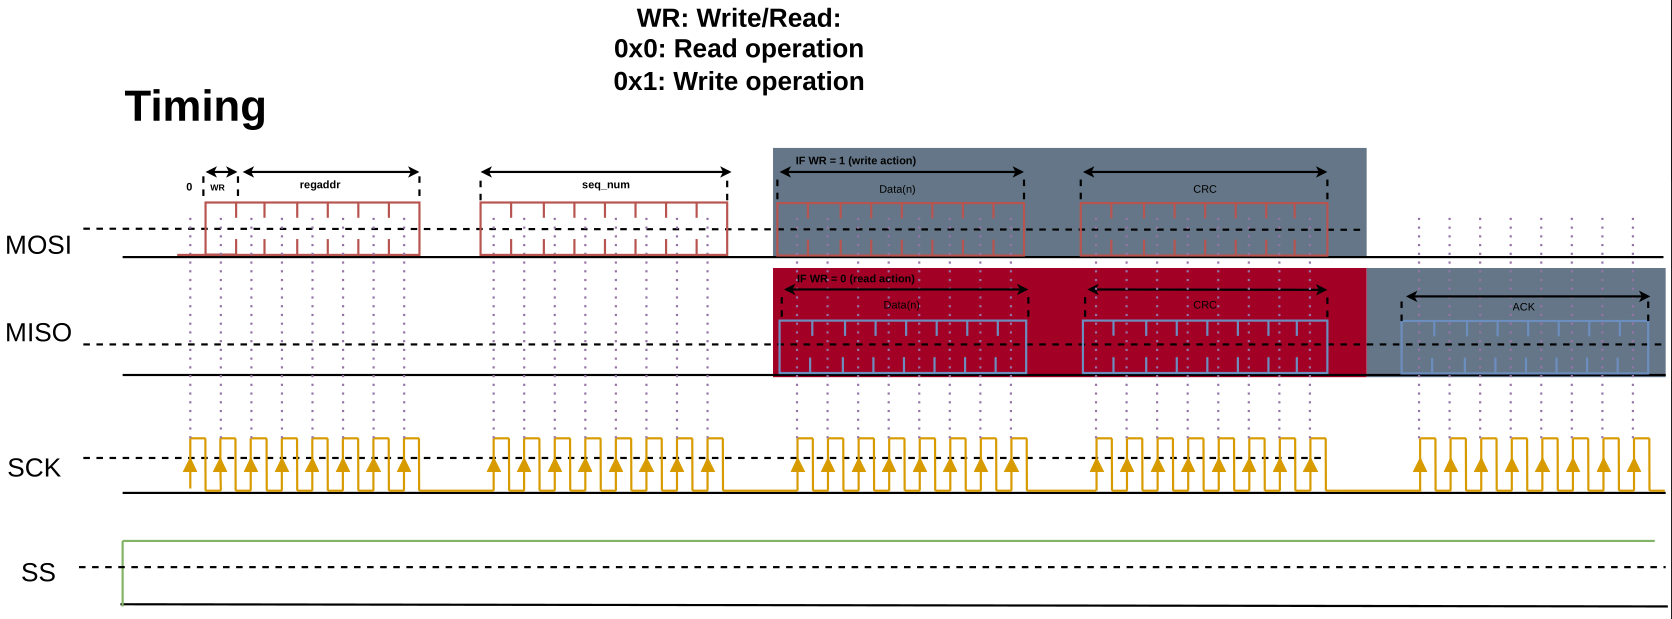
\includegraphics[scale=0.28]{figures/mainboard_communication_timing_diagram.png}
\pagebreak
\section{Registers}
This section will list all the registers of the mainboard.
\subsection{Register STATUS}
regaddr: 0x00\\
Register size: 32-bits\\
R/W: R\\
\begin{table}[h!]
    \centering
\begin{tabular}{rp{1.25cm}p{1.25cm}p{1.25cm}p{1.25cm}p{1.25cm}p{1.25cm}p{1.25cm}p{1.25cm}}
Bit &
  31 &
  30 &
  29 &
  28 &
  27 &
  26 &
  25 &
  24 \\ \cline{2-9} 
\multicolumn{1}{r|}{} &
  \multicolumn{1}{c|}{\scriptsize{BBAOK}} &
  \multicolumn{1}{c|}{\scriptsize{BBBOK}} & 
  \multicolumn{1}{c|}{\scriptsize{BBCOK}} &
  \multicolumn{1}{c|}{\scriptsize{BBDOK}} &
  \multicolumn{1}{c|}{\scriptsize{x}} &
  \multicolumn{1}{c|}{\scriptsize{x}} &
  \multicolumn{1}{c|}{\scriptsize{BLOK}} &
  \multicolumn{1}{c|}{\scriptsize{I2COK}} \\\cline{2-9} 
Access &
  R &
  R &
  R &
  R &
  R &
  R &
  R &
  R
\end{tabular}
\begin{tabular}{rp{1.25cm}p{1.25cm}p{1.25cm}p{1.25cm}p{1.25cm}p{1.25cm}p{1.25cm}p{1.25cm}}
Bit &
  23 &
  22 &
  21 &
  20 &
  19 &
  18 &
  17 &
  16 \\ \cline{2-9} 
\multicolumn{1}{r|}{} &
  \multicolumn{1}{c|}{\scriptsize{BAPAOK}} &
  \multicolumn{1}{c|}{\scriptsize{BAPBOK}} & 
  \multicolumn{1}{c|}{x} &
  \multicolumn{1}{c|}{\scriptsize{BBPAOK}} &
  \multicolumn{1}{c|}{\scriptsize{BBPBOK}} &
  \multicolumn{1}{c|}{x} &
  \multicolumn{1}{c|}{\scriptsize{BCPAOK}} &
  \multicolumn{1}{c|}{\scriptsize{BCPBOK}} \\\cline{2-9} 
Access &
  R &
  R &
  R &
  R &
  R &
  R &
  R &
  R
\end{tabular}
\begin{tabular}{rp{1.25cm}p{1.25cm}p{1.25cm}p{1.25cm}p{1.25cm}p{1.25cm}p{1.25cm}p{1.25cm}}
Bit &
  15 &
  14 &
  13 &
  12 &
  11 &
  10 &
  9 &
  8 \\ \cline{2-9} 
\multicolumn{1}{r|}{} &
  \multicolumn{1}{c|}{x} &
  \multicolumn{1}{c|}{\scriptsize{BDPAOK}} & 
  \multicolumn{1}{c|}{\scriptsize{BDPBOK}} &
  \multicolumn{1}{c|}{\scriptsize{x}} &
  \multicolumn{1}{c|}{\scriptsize{x}} &
  \multicolumn{1}{c|}{x} &
  \multicolumn{1}{c|}{\scriptsize{x}} &
  \multicolumn{1}{c|}{\scriptsize{x}} \\\cline{2-9} 
Access &
  R &
  R &
  R &
  R &
  R &
  R &
  R &
  R
\end{tabular}

\begin{tabular}{rp{1.25cm}p{1.25cm}p{1.25cm}p{1.25cm}p{1.25cm}p{1.25cm}p{1.25cm}p{1.25cm}}
Bit &
  7 &
  6 &
  5 &
  4 &
  3 &
  2 &
  1 &
  0 \\ \cline{2-9} 

\multicolumn{1}{r|}{x} &
  \multicolumn{1}{c|}{x} &
  \multicolumn{1}{c|}{x} & 
  \multicolumn{1}{c|}{x} &
  \multicolumn{1}{c|}{x} & 
  \multicolumn{1}{c|}{x} & 
  \multicolumn{1}{c|}{x} &
  \multicolumn{1}{c|}{x} &
  \multicolumn{1}{c|}{x} \\\cline{2-9} 
  
Access &
  R &
  R &
  R &
  R &
  R &
  R &
  R &
  R
\end{tabular}
\end{table}\\
\textbf{Bit 31 - BBAOK} Backbone port A status\\\\
\begin{tabular}{|c|l|}
    \hline
   BBAOK & Description\\ \hline
   0x0 & Backbone port disabled\\ \hline
   0x1 & Backbone port initialized succesfully \\ \hline
\end{tabular}\\\\
\textbf{Bit 30 - BBBOK} Backbone port B status\\\\
\begin{tabular}{|c|l|}
    \hline
   BBBOK & Description\\ \hline
   0x0 & Backbone port disabled\\ \hline
   0x1 & Backbone port initialized succesfully \\ \hline
\end{tabular}\\\\
\textbf{Bit 29 - BBCOK} Backbone port C status\\\\
\begin{tabular}{|c|l|}
    \hline
   BBCOK & Description\\ \hline
   0x0 & Backbone port disabled\\ \hline
   0x1 & Backbone port initialized succesfully \\ \hline
\end{tabular}\\\\
\textbf{Bit 28 - BBDOK} Backbone port D status\\\\
\begin{tabular}{|c|l|}
    \hline
   BBDOK & Description\\ \hline
   0x0 & Backbone port disabled\\ \hline
   0x1 & Backbone port initialized succesfully \\ \hline
\end{tabular}\\\\
\textbf{Bit 25 - BLOK} Bluetooth status\\\\
\begin{tabular}{|c|l|}
    \hline
   BLOK & Description\\ \hline
   0x0 & Bluetooth disabled\\ \hline
   0x1 & Bluetooth initialized succesfully and active\\ \hline
\end{tabular}\\\\
\pagebreak\\
\textbf{Bit 24 - I2COK} I2C status\\\\
\begin{tabular}{|c|l|}
    \hline
   I2COK & Description\\ \hline
   0x0 & I2C bus disabled\\ \hline
   0x1 & I2C bus initialized succesfully \\ \hline
\end{tabular}\\\\
\textbf{Bit 23 - BAPAOK} Backbone A SensorHub/ActuatorHub port A status\\\\
\begin{tabular}{|c|l|}
    \hline
   BAPAOK & Description\\ \hline
   0x0 & Sensor or Actuatorport disabled\\ \hline
   0x1 & Sensor or Actuatorport initialized succesfully and active\\ \hline
\end{tabular}\\\\
\textbf{Bit 22 - BAPBOK} Backbone A SensorHub/ActuatorHub port B status\\\\
\begin{tabular}{|c|l|}
    \hline
   BAPBOK & Description\\ \hline
   0x0 & Sensor or Actuatorport disabled\\ \hline
   0x1 & Sensor or Actuatorport initialized succesfully and active\\ \hline
\end{tabular}\\\\
\textbf{Bit 20 - BBPAOK} Backbone B SensorHub/ActuatorHub port A status\\\\
\begin{tabular}{|c|l|}
    \hline
   BBPAOK & Description\\ \hline
   0x0 & Sensor or Actuatorport disabled\\ \hline
   0x1 & Sensor or Actuatorport initialized succesfully and active\\ \hline
\end{tabular}\\\\
\textbf{Bit 19 - BBPBOK} Backbone B SensorHub/ActuatorHub port B status\\\\
\begin{tabular}{|c|l|}
    \hline
   BBPBOK & Description\\ \hline
   0x0 & Sensor or Actuatorport disabled\\ \hline
   0x1 & Sensor or Actuatorport initialized succesfully and active\\ \hline
\end{tabular}\\\\
\textbf{Bit 17 - BCPAOK} Backbone C SensorHub/ActuatorHub port A status\\\\
\begin{tabular}{|c|l|}
    \hline
   BCPAOK & Description\\ \hline
   0x0 & Sensor or Actuatorport disabled\\ \hline
   0x1 & Sensor or Actuatorport initialized succesfully and active\\ \hline
\end{tabular}\\\\
\textbf{Bit 16 - BCPBOK} Backbone C SensorHub/ActuatorHub port B status\\\\
\begin{tabular}{|c|l|}
    \hline
   BCPBOK & Description\\ \hline
   0x0 & Sensor or Actuatorport disabled\\ \hline
   0x1 & Sensor or Actuatorport initialized succesfully and active\\ \hline
\end{tabular}\\\\
\textbf{Bit 14 - BDPAOK} Backbone D SensorHub/ActuatorHub port A status\\\\
\begin{tabular}{|c|l|}
    \hline
   BDPAOK & Description\\ \hline
   0x0 & Sensor or Actuatorport disabled\\ \hline
   0x1 & Sensor or Actuatorport initialized succesfully and active\\ \hline
\end{tabular}\\\\
\textbf{Bit 13 - BDPBOK} Backbone D SensorHub/ActuatorHub port B status\\\\
\begin{tabular}{|c|l|}
    \hline
   BDPBOK & Description\\ \hline
   0x0 & Sensor or Actuatorport disabled\\ \hline
   0x1 & Sensor or Actuatorport initialized succesfully and active\\ \hline
\end{tabular}\\\\
\subsection{Register BBSETx}
regaddr: 0x01 + backbone\_port\_index (0x01-0x04)\\
Example: backbone port a: 0x01, port b: 0x02\\
Register size: 24-bits\\
R/W: RW\\
\begin{table}[h!]
    \centering
\begin{tabular}{rp{1cm}p{1cm}p{1cm}p{1cm}p{1cm}p{1cm}p{1cm}p{1cm}}
Bit &
  31 &
  30 &
  29 &
  28 &
  27 &
  26 &
  25 &
  24 \\ \cline{2-9} 
\multicolumn{1}{r|}{} &
  \multicolumn{2}{c}{} &
   \multicolumn{1}{c}{} &
  \multicolumn{2}{l}{\scriptsize{SLADDR[8:0]}} &
  \multicolumn{1}{c}{} &
  \multicolumn{1}{c}{} &
  \multicolumn{1}{c|}{} \\\cline{2-9} 
Access &
  R/W &
  R/W &
  R/W &
  R/W &
  R/W &
  R/W &
  R/W &
  R/W
\end{tabular}
\begin{tabular}{rp{1cm}p{1cm}p{1cm}p{1cm}p{1cm}p{1cm}p{1cm}p{1cm}}
Bit &
  23 &
  22 &
  21 &
  20 &
  19 &
  18 &
  17 &
  16 \\ \cline{2-9} 
\multicolumn{1}{r|}{} &
\multicolumn{4}{c|}{\scriptsize{PASAMPLETIME[4:0]}} & 
\multicolumn{4}{c|}{\scriptsize{PBSAMPLETIME[4:0]}} \\\cline{2-9} 
Access &
  R/W &
  R/W &
  R/W &
  R/W &
  R/W &
  R/W &
  R/W &
  R/W
\end{tabular}
\begin{tabular}{rp{1cm}p{1cm}p{1cm}p{1cm}p{1cm}p{1cm}p{1cm}p{1cm}}
Bit &
  15 &
  14 &
  13 &
  12 &
  11 &
  10 &
  9 &
  8 \\ \cline{2-9} 
  
\multicolumn{1}{r|}{} &
  \multicolumn{2}{c|}{{\scriptsize{BBTYPE[1:0]}}} &
  \multicolumn{2}{c}{} &
  \multicolumn{2}{c}{{\scriptsize{PATYPE[6:0]}}} &
  \multicolumn{1}{c}{} &
  \multicolumn{1}{c|}{} \\\cline{2-9} 
Access &
  R/W &
  R/W &
  R/W &
  R/W &
  R/W &
  R/W &
  R/W &
  R/W
\end{tabular}
\begin{tabular}{rp{1cm}p{1cm}p{1cm}p{1cm}p{1cm}p{1cm}p{1cm}p{1cm}}
Bit &
  7 &
  6 &
  5 &
  4 &
  3 &
  2 &
  1 &
  0 \\ \cline{2-9} 

  \multicolumn{1}{r|}{} &
  \multicolumn{2}{c}{} &
  \multicolumn{2}{c}{\scriptsize{PBTYPE[6:0]}} &
  \multicolumn{2}{c|}{} &
  \multicolumn{1}{c|}{x} &
  \multicolumn{1}{c|}{\scriptsize{ENA}} \\\cline{2-9} 
  
Access &
  R/W &
  R/W &
  R/W &
  R/W &
  R/W &
  R/W &
  R/W &
  R/W
\end{tabular}
\end{table}\\
\textbf{Bits 31:24 - SLADDR[8:0]} I2C Slave address\\
This bit field defines the slave address of the to the backbone port connected slave device.\\\\
\textbf{Bits 23:20 - PASAMPLETIME[4:0]} Backbone slave port sample time or time base, 1-32 Ms\\
This bit field defines the sample time of port A of the slave device connected to Backbone x.\\\\
\textbf{Bits 23:20 - PBSAMPLETIME[4:0]} Backbone slave port sample time or time base, 1-32 Ms\\
This bit field defines the sample time of port B of the slave device connected to Backbone x.\\\\
\textbf{Bits 15:14 - BBTYPE[1:0]} Backbone slave device type\\
This bit field defines the slave device type connected to the backbone port.\\\\
\begin{tabular}{|c|l|l|}
\hline
   BBTYPE[1:0]  &  Name & Description\\ \hline
    0x0 &  SensorHub & SensorHub slave\\ \hline
    0x1 & ActuatorHub & ActuatorHub slave\\ \hline
    0x2 & Reserved & Reserved for future use\\ \hline
    0x3 & Reserved & Reserved for future use\\
\hline
\end{tabular}\\\\\\
\textbf{Bits 13:8 - PATYPE[6:0]} PORTA Type\\
This bit field defines the sensors or actuators connected to PORT A of the SensorHub or
ActuatorHub.\\\\
\begin{tabular}{|c|l|l|}
    \hline
    PATYPE[6:0] & Name & Description \\ \hline
    0x00 & None & No sensor is connected\\ \hline
    0x01 & ToF & A time of flight sensor is connected\\ \hline
    0x02 & DiffPressure & A differential pressure sensor is connected\\ \hline
    0x03 & TouchSensor & A thoraxtouch sensor is connected\\ \hline
    0x04 & Gyro & A gyro sensor is connected\\ \hline
    0x05..0x20 & Reserved & Reserved for future use\\ \hline
    0x21 & Pump & A pump actuator is connected\\ \hline
    0x22..0x40 & Reserved & Reserved for future use \\ \hline
\end{tabular}
\\\\
\textbf{Bits 7:2 - PBTYPE[6:0]} PORTB Type\\
This bit field defines the sensors or actuators connected to PORT B of the SensorHub or
ActuatorHub.\\\\
\begin{tabular}{|c|l|l|}
    \hline
    PBTYPE[6:0] & Name & Description \\ \hline
    0x00 & None & No sensor is connected\\ \hline
    0x01 & ToF & A time of flight sensor is connected\\ \hline
    0x02 & DiffPressure & A differential pressure sensor is connected\\ \hline
    0x03 & TouchSensor & A thoraxtouch sensor is connected\\ \hline
    0x04 & Gyro & A gyro sensor is connected\\ \hline
    0x05..0x20 & Reserved & Reserved for future use\\ \hline
    0x21 & Pump & A pump actuator is connected\\ \hline
    0x22..0x40 & Reserved & Reserved for future use \\ \hline
\end{tabular}
\\\\
\textbf{Bit 0 - ENA} Enable backbone port\\\\
\begin{tabular}{|c|c|}
    \hline
   ENA & Description\\ \hline
   0x0 & Backbone port disabled\\ \hline
   0x1 & Backbone port enabled \\ \hline
\end{tabular}

\pagebreak

\subsection{Register REQWORDSx}
regaddr: 0x10 + backbone\_port\_index (0x10-0x14)\\
Example: backbone port a: 0x10, port b: 0x11\\
Register size: 24-bits\\
R/W: RW\\
\begin{table}[h!]
    \centering
\begin{tabular}{rp{1.25cm}p{1.25cm}p{1.25cm}p{1.25cm}p{1.25cm}p{1.25cm}p{1.25cm}p{1.25cm}}
Bit &
  23 &
  22 &
  21 &
  20 &
  19 &
  18 &
  17 &
  16 \\ \cline{2-9} 
\multicolumn{1}{r|}{} &
 \multicolumn{8}{c|}{\scriptsize{BxREQWORDS[7:0]}} \\\cline{2-9} 
Access &
  R/W &
  R/W &
  R/W &
  R/W &
  R/W &
  R/W &
  R/W &
  R/W 
\end{tabular}
\begin{tabular}{rp{1.25cm}p{1.25cm}p{1.25cm}p{1.25cm}p{1.25cm}p{1.25cm}p{1.25cm}p{1.25cm}}
Bit &
  15 &
  14 &
  13 &
  12 &
  11 &
  10 &
  9 &
  8 \\ \cline{2-9} 
\multicolumn{1}{r|}{} &
  \multicolumn{8}{c|}{\scriptsize{BxREQWORDSPA[7:0]}}  \\\cline{2-9} 
Access &
  R/W &
  R/W &
  R/W &
  R/W &
  R/W &
  R/W &
  R/W &
  R/W 
\end{tabular}

\begin{tabular}{rp{1.25cm}p{1.25cm}p{1.25cm}p{1.25cm}p{1.25cm}p{1.25cm}p{1.25cm}p{1.25cm}}
Bit &
  7 &
  6 &
  5 &
  4 &
  3 &
  2 &
  1 &
  0 \\ \cline{2-9} 

\multicolumn{1}{r|}{x} &
  \multicolumn{8}{c|}{\scriptsize{BxREQWORDSPB[7:0]}}  \\\cline{2-9} 
  
Access &
  R/W &
  R/W &
  R/W &
  R/W &
  R/W &
  R/W &
  R/W &
  R/W 
\end{tabular}
\end{table}\\
\textbf{Bits 23:16 - BxREQWORDS[7:0]} Backbone x REQWORDS\\
This bitfield has the sum of the BxREQWORDSPA and BxREQWORDSPB register. This bitfield will be read-only when the backbone slave device is a SensorHub otherwise it will be read/write.\\\\
\textbf{Bits 15:8 - BxREQWORDSPA[7:0]} Backbone x Slave Port A REQWORDS\\
This bitfield is the amount of bytes that gets out of the sensor on Port A or needs to be provided to an actuator on Port A. \\
This bitfield will be read-only when the backbone slave device is a SensorHub otherwise it will be read/write.\\\\
\textbf{Bits 8:0 - BxREQWORDSPB[7:0]} Backbone x Slave Port B REQWORDS\\
This bitfield is the amount of bytes that gets out of the sensor on Port B or needs to be provided to an actuator on Port B. \\
This bitfield will be read-only when the backbone slave device is a SensorHub otherwise it will be read/write.
\subsection{Register SENSDATA}
regaddr: 0x30\\
Register size: n-bits (depends on sensor) can be read from REQWORDS reg\\
R/W: R\\
\\
\textbf{The bits returned will be raw sensordata.. The layout is always in alphabetical order and depends on the sensors}
\subsection{Register ACTDATA}
regaddr: 0x40\\
Register size: n-bits can be set in the REQWORDS reg, default value will be defined by the actuatorhub\\
R/W: W\\
\\
\textbf{The bits that need to be written will be raw actuatordata.. The layout is always in alphabetical order and depends on the actuators and bits set in REQWORDSx reg}


    \chapter{USB service protocol}
\section{Introduction}
For the communication bus over the usb service port on the mainboard, sensorhubs and actuatorhub is a well described datacommunication protocol needed. This chapter will provide the information needed to implement the datacommunication protocol used over the usb service port in software/hardware.
\section{Underlying interfacemethod}
The underlying datacommunication interface will be UART over USB (VCOM). UART was chosen because of ease of use. This protocol is widely supported on multiple platforms and easy to setup within the framework used on the mainboard/hubs.
\section{Protocol specification}
UART itself leaves a lot to be filled in by the protocol on top. This offers great flexibility, however it also takes a lot of work and documentation to get it consistent. This section is dedicated to give general specifications of the data protocol used.

\section{Timing diagram}

\def\degr{${}^\circ$}
\begin{tikztimingtable}
  Clock 128\,MHz 0\degr    & H 2C N(A1) 8{2C} N(A5) 3{2C} G\\
  Clock 128\,MHz 90\degr   & [C] 2{2C} N(A2) 8{2C} N(A6) 2{2C} C\\
  Clock 128\,MHz 180\degr  & C 2{2C} N(A3) 8{2C} N(A7) 2{2C} G\\
  Clock 128\,MHz 270\degr  & 3{2C} N(A4) 8{2C} N(A8) 2C C\\
  Coarse Pulse             & 3L 16H 6L \\
  Coarse Pulse - Delayed 1 & 4L N(B2) 16H N(B6) 5L \\
  Coarse Pulse - Delayed 2 & 5L N(B3) 16H N(B7) 4L \\
  Coarse Pulse - Delayed 3 & 6L 16H 3L \\
  \\
  Final Pulse Set          & 3L 16H N(B5) 6L \\
  Final Pulse $\overline{\mbox{Reset}}$ & 6L N(B4) 16H 3L \\
  Final Pulse              & 3L N(B1) 19H N(B8) 3L \\
\extracode
  \tablerules
  \begin{pgfonlayer}{background}
    \foreach \n in {1,...,8}
      \draw [help lines] (A\n) -- (B\n);
  \end{pgfonlayer}
\end{tikztimingtable}
    \chapter{Log Script Manual}
The log script is developed for the purpose to process the data stream of the usb service port. The script creates a csv log file and also a Excel file as a table.

\textbf{To run the script:}
\begin{itemize}
  \item Make sure you have Python installed. 
  Open your terminal and type "Python", if Python is installed you can find the version. 
  \item Also the script needs the following external packages: Pandas and pyserial. \\
  To install these you can type "python install pandas pyserial".
  \item Select the COM port or serial port of the hub that you want to log the stream of. \\
 \begin{figure}[h!]
  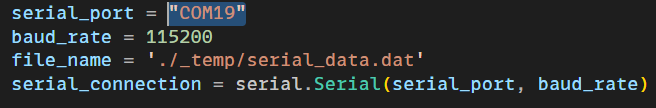
\includegraphics{figures/Script COM selection.png}
  \caption{Script USB Configuration}
  \end{figure}
 \item Run the script by typing: "python -u main.py" in the script fileLogger folder. 
\end{itemize}
\end{document}
